%\label{Model_Selection}

Selecting the best model to represent a process is often not a trivial task. This chapter discusses methods of comparing models against data, approximating parameters, and testing whether a model fits. 

\section{Maximum Likelihood Estimators}
\label{Model_Selection:Maximum_Liklihood_Estimators}

We wish to find a model that can explain a given dataset. Assume we have two such models; how do we decide which is superior at this task? In this chapter, we will build on this idea. 

    \subsection{Likelihood}
    \label{Model_Selection:Maximum_Liklihood_Estimators:Likelihood}

    In this subsection, we define likelihood and motivate the need for Maximum likelihood estimators.

    To decide between models, we must answer which model explains the dataset better. We interpret this as the probability a given model produces a sequence of observations. This probability is known as the likelihood. We can now define this; \cite{Ross2004}.

    \begin{definition} Likelihood Function \\
        Given model $\theta$ and the observations $x_1, x_2,...,x_n$, the likelihood function is given by
        \begin{equation}
            \label{Definition:Likelihood}
            L(\theta|x_1, x_2,...,x_n) = \prob(x_1, x_2,...,x_n|\theta)
        \end{equation} 
        In other words it is given by the probability that the given model produced the given observations.
    \end{definition}

    This function allows us to directly compare which model has a higher probability of fitting the data. A model with a higher Likelihood would have a superior fit to a model with a lower likelihood. As such, it is natural to maximise the likelihood in search of the ideal model. 

    \subsection{Maximum Liklihood Estimators}
    \label{Model_Selection:Maximum_Liklihood_Estimators:MLE}

    Through maximising the likelihood function \ref{Definition:Likelihood}, we can find the model that best fits the given observations. This process is called Maximum Likelihood estimation. In this subsection, we will demonstrate its methodology.

    We often use log$(L(\theta|x_1, x_2,...,x_n))$ instead of $L(\theta|x_1, x_2,...,x_n)$ as this often leads to easier differenciation. This is possible as the log function is monotonically increassing thus has the same maximum at the same value of $\theta$.

    The method can be described as follows:
    \begin{enumerate}[i]
        \label{Model_Selection:Maximum_Liklihood_Estimators:MLE:Method}
        \item Calculate the joint probability density of observeriving your data $X_1 = x_1,...,X_n=x_n$ given your model $\theta$, i.e.
        \begin{equation}
            \prob(X_1 = x_1,...,X_n=x_n|\theta)
        \end{equation}
        \item Take the Natural logarithm of both sides. 
        \begin{equation}
            \ln(\prob(X_1 = x_1,...,X_n=x_n|\theta))
        \end{equation}
        \item Take the partial derivative with respect to each parameter.
        \item For each paramter, set the derivative equal to 0 and rearrange for its value. The given value will be the maximum likelihood estimation of that parameter.
    \end{enumerate}

    \begin{example}
        \label{Model_Selection:Maximum_Liklihood_Estimators:MLE:Example}
        To demonstrate \ref{Model_Selection:Maximum_Liklihood_Estimators:MLE:Method} we present the following example. 

        Let $\{1,2,4,4,4,9\}$ be our Observed data. We are convived that this data follows an expoential($\lambda$) distribution but we are unsure of what the $\lambda$ parameter is. We begin by finding the joint probability density. According to our model all observations are independent thus the joint distribution is:
        \begin{equation}
            \prob(X_1 = x_1,...,X_6=x_6|\theta) = \prob(X_1 = x_1)...\prob(X_6 = x_6)
        \end{equation}

        We can now substitute in the PDF of an expoential distribtution at the different observations.
        \begin{equation}
            \prob(X_1 = x_1,...,X_6=x_6|\theta) = \lambda e^{-\lambda} \lambda e^{-2\lambda} \lambda e^{-4\lambda} \lambda e^{-4\lambda} \lambda e^{-4\lambda} \lambda e^{-9\lambda}
        \end{equation}

        We now simplify and take the natural log of both sides.
        \begin{eqnarray}
            \ln(\prob(X_1 = x_1,...,X_6=x_6|\theta)) & = &  \ln(\lambda^6 e^{-24\lambda}) \\
            & = & ln(\lambda^6) - 24\lambda 
        \end{eqnarray}

        We now differenciate with respect to our parameter, $\lambda$.
        \begin{equation}
            \dfrac{d}{d\lambda} = \dfrac{6}{\lambda} - 24
        \end{equation}

        Finally, to find the maximum we set the differential equal to 0 and solve for $\lambda$.
        \begin{eqnarray}
            0 & = & \dfrac{6}{\lambda} - 24 \\
            24 & = & \dfrac{6}{\lambda} \\
            \lambda & = & \dfrac{6}{24} \\
            & = & \dfrac{1}{4}    
        \end{eqnarray}

        Through MLE, our parameter estimate for $\lambda$ is 0.25; thus our model is exponential(0.25). Logically this seems to make sense as the expected value of this model is 4, which seems to be the most popular and central value from the dataset.
    \end{example}


    As we can see, even for a simple model, the derivate is not trivial. Unfortunately, in real-world applications, this is often the case, particularly true for Hidden Markov based models. Thus we often require alternative methods to compare models.


\section{Approximate Bayesian Computation}
\label{Model_Selection:Approximate_Bayesian_Computation}

Maximum Likelihood Estimators are not always easy to calculate. Approximate Bayesian Computation (ABC) can provide an alternative method of parameter estimation in some such cases. In this section, we will discuss the principles of Bayesian Statistics, ABC and provide a demonstration.

ABC uses Bayesian inference. It involves using the prior distribution, our assumption of the model, combined with the likelihood to infer a posterior distribtution, the expected distribtution given our data and model. This can be more formally described using Bayes Theorem. Given $x$ is the data and $\theta$ is the model, 
\begin{eqnarray}
    \prob(\theta|x) & = & \dfrac{\prob(x|\theta)\prob(\theta)}{\prob(x)} \\
    \prob(\theta|x) & \propto & \prob(x|\theta)\prob(\theta) \\
    posterior  & \propto & likelihood * prior
\end{eqnarray}

ABC infers posterior distributions by replacing the likelihood calculation with a comparison between observed and simulated data. \cite{Toni2009}. While there are many variations of ABC, we will focus on the simplest, ABC Rejection Sampling. The method can is as follows:

\begin{enumerate}
    \label{Model_Selection:Approximate_Bayesian_Computation:Method}
    \item Sample $\theta'$ from the prior distribution $\prob(\theta)$.
    \item Simulate dataset $x'$ using the sampled $\theta'$.
    \item Compare simulated dataset with observed dataset using a distance function. If the distance is smaller than a preset $\epsilon$, then accept $\theta'$; otherwise, reject. The distance function can use summary statistics.
    \item Repeat previous steps.
\end{enumerate}

Given a small enough tolerence ($\epsilon$) and an appropriate statistic we have:
\begin{equation}
    \label{Model_Selection:Approximate_Bayesian_Computation:posterior_convergence}
    \prob_{\epsilon}(\theta|x) = \int \prob_{\epsilon}(\theta, x'|x)dx' \approx \prob(\theta|x)
\end{equation}

\begin{example}
    \label{Model_Selection:Approximate_Bayesian_Computation:Example}
    To demonstrate ABC, we will set the posterior distribtution and attempt to sample from it indirectly.

    Let our observation data be 10000 Poisson(5) random variables. Also, let our prior distribution be Poisson(10). In other words, the actual distribution (posterior distribution) is Poisson(5), but we believe it is Poisson(10). Let our summary statistics be mean and variance, both of which must be within $\epsilon =1$ difference between simulated and actual. Code for this example is available in the "Example" folder under "MyCode" in the "ABC.R" file.

    We begin with the first step of \ref{Model_Selection:Approximate_Bayesian_Computation:Method}. We generate a Poisson(10) variable $\theta'$. Now we simulate Poisson($\theta')$. If the mean and variance of this sample are within 1 of the mean and variance for the observation data we accept, else we reject. We generate simulations of size 10000 in order to generate 1000 random variables distributed by our posterior distribution. 

    \begin{figure}
        \centering
        \begin{subfigure}{.45\textwidth}
            \centering
            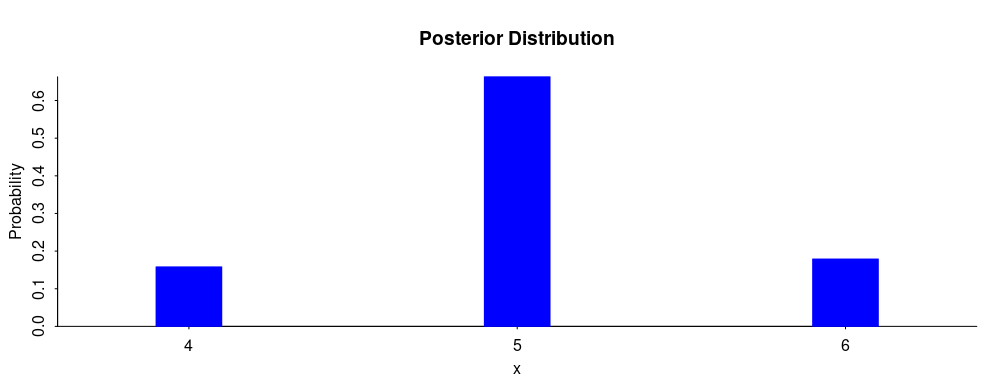
\includegraphics[width=\linewidth]{ABC example/posterior.png}
            \caption{Posterior Distribtution}
            \label{Model_Selection:Approximate_Bayesian_Computation:Example_Figure:1}
        \end{subfigure}
        \begin{subfigure}{.45\textwidth}
            \centering
            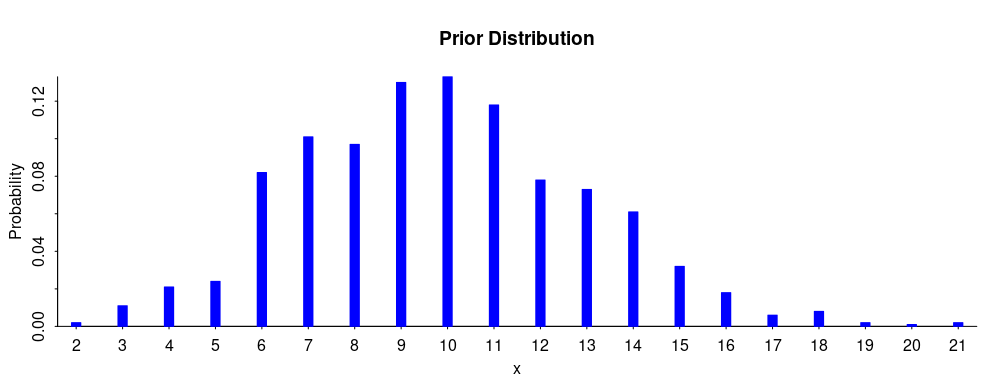
\includegraphics[width=\linewidth]{ABC example/prior.png}
            \caption{Prior Distribtution}
            \label{Model_Selection:Approximate_Bayesian_Computation:Example_Figure:2}
        \end{subfigure}    

        \begin{subfigure}{.45\textwidth}
            \centering
            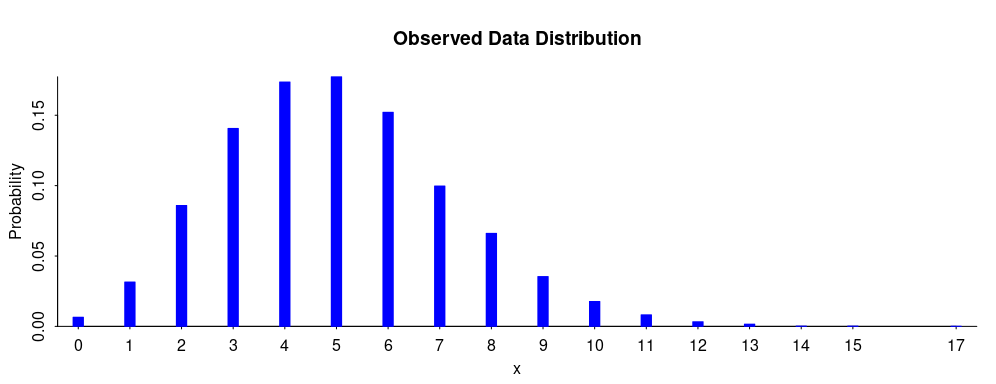
\includegraphics[width=\linewidth]{ABC example/data.png}
            \caption{Observation Data Distribtution }
            \label{Model_Selection:Approximate_Bayesian_Computation:Example_Figure:3}
        \end{subfigure}
        \caption{A graphical reprsentation of the posteior, prior and observed distributions for Example \ref{Model_Selection:Approximate_Bayesian_Computation:Example}.}
        \label{Model_Selection:Approximate_Bayesian_Computation:Example_Figure}
    \end{figure} 

    As we can see from Figure \ref{Model_Selection:Approximate_Bayesian_Computation:Example_Figure}, the ABC generated sample has sampled from the high probability density areas of the true distribution. To get a complete posterior, which accounts for extreme values with lower probability, one should investigate other summary statistics.
\end{example}




\section{Kolmogorov-Smirnov Test}
\label{Model_Selection:Kolmogorov_Smirnov_Test}

This section will introduce a method to compare the similarity between two sets of data; the Kolmogorov-Smirnov Test.

Once we have a model, we must test to see how effective it is as generating values that follow the observed distribution. One such test for continuously distributed data is the Kolmogorov-Smirnov test. This test is a form of hypothesis testing. 

Suppose we have two sets of data, our observed and simulated. We begin by calculating the empirical cumulative distribution function for each. We will label these as $F_o$ for observed and $F_s$ for simulated data. We can now state the hypothesis.

\begin{itemize}
    \item $H_0$ := $F_o = F_s$, the two datasets are distributed by the same distribtution.
    \item $H_1$ := $F_o \neq F_s$, the two datasets are not distributed by the same distributed. 
\end{itemize}

The test statistic is given by the following:
\begin{equation}
    D \equiv Max_x |F_s(x) - F_o(x)|
\end{equation}

The P-value is calculated using a probability of this test statistic. We will not explore this in-depth, but more information can be found at \cite{Ross2004}[506]. If the P-value is smaller than the selected significance level, then we reject the null hypothesis. Otherwise, we say we have insufficient evidence to reject. 

If we reject the null hypothesis, then our model is incorrect. If we do not reject, then our model may produce simulations matching in distribution to the observed data.
